\documentclass[12pt,a4paper]{article}
%\title{Software Requirements Specification}
%\date{December 14, 2015}
%\author{Aven Bross}
\usepackage[latin1]{inputenc}
\usepackage{amsmath}
\usepackage{amsfonts}
\usepackage{amssymb}
\usepackage{amsthm}
\usepackage{enumitem}
\usepackage[english]{babel}
\usepackage{fancyhdr}
\usepackage{chngpage}
\usepackage{geometry}
\usepackage{tabularx}
\usepackage{algorithm2e}
\usepackage[dvipsnames]{xcolor}
\geometry{legalpaper, portrait, margin=1.25in}

\usepackage{tikz}

\usepackage [autostyle, english = american]{csquotes}
\MakeOuterQuote{"}

\pagenumbering{gobble}

\begin{document}

\begin{center}

\tikzset{every loop/.style={min distance=1cm,in=-15,out=45,looseness=15}}

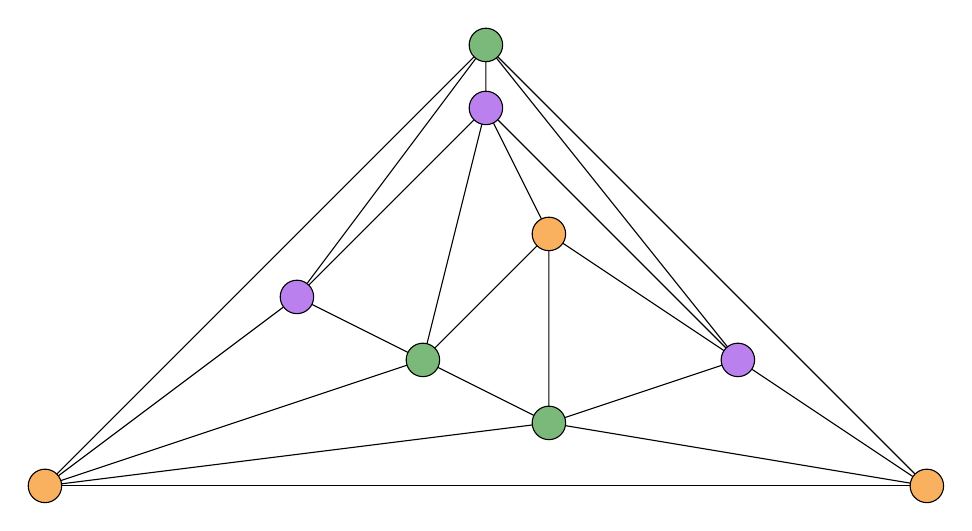
\begin{tikzpicture}[scale=.8, every node/.style={circle, draw, minimum size=8.5mm, scale=.5}]
  \node [fill=BurntOrange!60] (0) at (0cm, 0cm) {$$};
  \node [fill=BurntOrange!60] (1) at (14cm, 0cm) {$$};
  \node [fill=BlueViolet!60] (2) at (11cm, 2cm) {$$};
  \node [fill=ForestGreen!60] (3) at (8cm, 1cm) {$$};
  \node [fill=BurntOrange!60] (4) at (8cm, 4cm) {$$};
  \node [fill=BlueViolet!60] (5) at (7cm, 6cm) {$$};
  \node [fill=ForestGreen!60] (6) at (6cm, 2cm) {$$};
  \node [fill=BlueViolet!60] (7) at (4cm, 3cm) {$$};
  \node [fill=ForestGreen!60] (8) at (7cm, 7cm) {$$};
  \draw (0) -- (1);
  \draw (0) -- (8);
  \draw (8) -- (1);
  \draw (2) -- (1);
  \draw (3) -- (1);
  \draw (2) -- (8);
  \draw (3) -- (0);
  \draw (2) -- (5);
  \draw (2) -- (4);
  \draw (2) -- (3);
  \draw (3) -- (6);
  \draw (3) -- (4);
  \draw (4) -- (5);
  \draw (4) -- (6);
  \draw (5) -- (8);
  \draw (5) -- (7);
  \draw (5) -- (6);
  \draw (6) -- (0);
  \draw (6) -- (7);
  \draw (7) -- (8);
  \draw (7) -- (0);
\end{tikzpicture}\\
\hfill\\
\hfill\\
\hfill\\

\begin{tikzpicture}[scale=.8, every node/.style={circle, draw, minimum size=8.5mm, scale=.5}]
  \node [fill=BurntOrange!60] (0) at (0cm, 0cm) {$$};
  \node [fill=BurntOrange!60] (1) at (14cm, 0cm) {$$};
  \node [fill=BurntOrange!60] (4) at (8cm, 4cm) {$$};
  \draw (0) -- (1);WWW
\end{tikzpicture}\\
\hfill\\
\hfill\\
\hfill\\

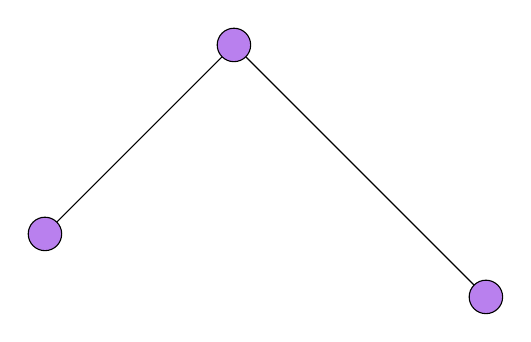
\begin{tikzpicture}[scale=.8, every node/.style={circle, draw, minimum size=8.5mm, scale=.5}]
  \node [fill=BlueViolet!60] (2) at (11cm, 2cm) {$$};
  \node [fill=BlueViolet!60] (5) at (7cm, 6cm) {$$};
  \node [fill=BlueViolet!60] (7) at (4cm, 3cm) {$$};
  \draw (5) -- (7);
  \draw (5) -- (2);
\end{tikzpicture}\\
\hfill\\
\hfill\\
\hfill\\

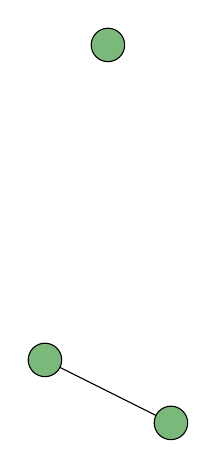
\begin{tikzpicture}[scale=.8, every node/.style={circle, draw, minimum size=8.5mm, scale=.5}]
  \node [fill=ForestGreen!60] (3) at (8cm, 1cm) {$$};
  \node [fill=ForestGreen!60] (6) at (6cm, 2cm) {$$};
  \node [fill=ForestGreen!60] (8) at (7cm, 7cm) {$$};
  \draw (3) -- (6);
\end{tikzpicture}\\
\hfill\\
\hfill\\
\hfill\\

\end{center}

\end{document}